\documentclass[11pt,a4paper,twoside]{article}

% LaTeX-Umsetzung der "Richtlinien f�r Projekt- und Diplomarbeiten"
% der LFE Medieninformatik, LMU M�nchen. (Autor: Richard Atterer, 27.9.2006, 23.10.2007), Bug-Fixing Mark Kaczkowski (23.6.2008)

\usepackage[T1]{fontenc} % sonst geht \hyphenation nicht mit Umlauten
\usepackage[latin1]{inputenc} % man kann schreiben ����, statt "a"o"u"s
%\usepackage[utf8]{inputenc} % wie oben, aber UTF-8 als Encoding statt ISO-8859-1 (latin1)
\usepackage[english]{babel} % deutsche Trennregeln, "Inhaltsverzeichnis" etc.
%\usepackage{ngerman} % Alternative zum Babel-Paket oben
\usepackage{mathptmx} % Times-Roman-Schrift (auch f�r mathematische Formeln)
\usepackage{enumitem} 
\usepackage{cite}

% Zum Setzen von URLs
\usepackage{color}
\definecolor{darkred}{rgb}{.25,0,0}
\definecolor{darkgreen}{rgb}{0,.2,0}
\definecolor{darkmagenta}{rgb}{.2,0,.2}
\definecolor{darkcyan}{rgb}{0,.15,.15}
\usepackage[plainpages=false,bookmarks=true,bookmarksopen=true,colorlinks=true,
  linkcolor=darkred,citecolor=darkgreen,filecolor=darkmagenta,
  menucolor=darkred,urlcolor=darkcyan]{hyperref}

% pdflatex: Bilder in den Formaten .jpeg, .png und .pdf
% latex: Bilder im .eps-Format
\usepackage{graphicx}

\usepackage{fancyhdr} % Positionierung der Seitenzahlen
\fancyhead[LE,RO,LO,RE]{}
\fancyfoot[CE,CO,RE,LO]{}
\fancyfoot[LE,RO]{\Roman{page}}
\renewcommand{\headrulewidth}{0pt}
\setlength{\headheight}{13.6pt} % behebt headheight Warning

% Korrektes Format f�r Nummerierung von Abbildungen (figure) und
% Tabellen (table): <Kapitelnummer>.<Abbildungsnummer>
\makeatletter
\@addtoreset{figure}{section}
\renewcommand{\thefigure}{\thesection.\arabic{figure}}
\@addtoreset{table}{section}
\renewcommand{\thetable}{\thesection.\arabic{table}}
\makeatother

\sloppy % Damit LaTeX nicht so viel �ber "overfull hbox" u.�. meckert

% R�nder
\addtolength{\topmargin}{-16mm}
\setlength{\oddsidemargin}{25mm}
\setlength{\evensidemargin}{35mm}
\addtolength{\oddsidemargin}{-1in}
\addtolength{\evensidemargin}{-1in}
\setlength{\textwidth}{15cm}
\addtolength{\textheight}{34mm}
%________________________________________________________

\begin{document}

\pagestyle{empty} % Vorerst keine Seitenzahlen
\pagenumbering{alph} % Unsichtbare alphabetische Nummerierung

\begin{center}
\textsc{Ludwig-Maximilians-Universit\"ut M\"unchen}\\
Department ``Institut f\"ur Informatik''\\
Lehr- und Forschungseinheit Medieninformatik\\
Prof. Dr. Florian Alt

\vspace{5cm}
{\large\textbf{Masterarbeit}}\vspace{.5cm}

{\LARGE Design and Development of a Public Display Survey Platform}\vspace{1cm}

{\large Lukas Ziegler}\\\href{mailto:lukas@lukasziegler.com}{lukas@lukasziegler.com}

\end{center}
\vfill

\begin{tabular}{ll}
Bearbeitungszeitraum: & 6.10.2014 bis 30.04.2015\\
Betreuer: & Prof. Dr. Florian Alt\\
Verantw. Hochschullehrer: & Prof. Dr. Florian Alt
\end{tabular}
%________________________________________________________

\clearpage

    
\section*{Zusammenfassung}

	In den letzten Jahren haben sich Public Displays (PD) in der {\"O}ffentlichkeit stark vermehrt und wurden Teil unseres t{\"a}glichen Lebens. In Einkaufszentren, Bahnh{\"o}fen und Flugh{\"a}fen gibt es immer mehr interaktive Anwendungen f{\"u}r PDs. Ihre Entwicklung erfordert eine umfassende Evaluation, was ein komplexes und zeitintensives Unterfangen ist. Bisher greifen viele der interaktiven Anwendungen noch nicht auf die M{\"o}glichkeit zur{\"u}ck, den R{\"u}ckkanal vom PD zum Display-Anbieter zu nutzen. Um dieses Problem zu l{\"o}sen wurde eine interaktive Umfrage-Plattform entwickelt und eine umfassende Literaturrecherche durchgef{\"u}hrt. \textit{PDSurvey} soll die Durchf{\"u}hrung von Umfragen auf Public Displays erleichtern und als Werkzeug zur weiteren Evaluierung dienen. In dieser Arbeit wird der Entwurf und die Entwicklung unserer Plattform vorgestellt und eine Liste an standardisierten Frageb{\"o}gen vorgeschlagen, welche aus einer umfangreichen Literaturrecherche resultieren. Au{\ss}erdem stellen wir die Ergebnisse unserer Feldstudie vor, in der wir untersucht haben wie Umfragen auf Public Displays wahrgenommen werden und welcher R{\"u}ckkanal am besten f{\"u}r den Nutzer geeignet ist um in digitaler Form auf einen Fragebogen zu antworten.
	Die Ergebnisse lassen folgern, dass eine Mehrheit der Nutzer es vorzieht Umfragen direkt vor Ort zu beantworten. Allerdings hat auch ein Viertel sich gegen die M{\"o}glichkeit entschieden, direkt vor Ort auf den Fragebogen zu antworten. Ein Tablet als R{\"u}ckkanal anzubieten hat sich als beste Option herausgestellt, auch wenn der Benutzer zwischen den Ger{\"a}ten wechseln muss. Umfragen welche direkt auf PDs durchgef{\"u}hrt werden stellen eine sinnvolle Alternative zu Online-Umfragen dar, mit der Einschr{\"a}nkung der sozialen Erw{\"u}nschtheit und der Abnahme der Privatsph{\"a}re.


\selectlanguage{english}
\section*{Abstract}

	In recent years, public displays (PD) have proliferated in public space and become part of our daily lives. New interactive applications for PDs are flourishing in shopping malls, train stations, and airports. Their development requires extensive evaluation, which is a complex and time intensive endeavor. So far, many interactive PDs still lack a feedback channel from display to display provider. To solve this problem an interactive survey platform was developed and an extensive literature review carried out.
	\textit{PDSurvey} aims to facilitate the execution of surveys on public displays and is a toolset for further PD evaluation. In this thesis, the design and development process of our platform is presented and a list of standardized questionnaires proposed, resulting from an extensive literature review. Furthermore, we present the findings of our field study, in which we assessed the general acceptance of questionnaires being conducted in public space and which feedback channels are best suited for users to respond to questionnaires in a digital form.
	The findings imply that a majority of users prefer to complete a survey directly on-site. However, a quarter refrained from using PDs for responding to the questionnaire. Offering the tablet as a feedback channel represented the best choice, even though users have to switch devices. Surveys conducted on public displays are a reasonable alternative to online surveys, with the limitation of social desirability and a decrease in privacy.
	


	% BENEFITS: simplifying evaluation, better scalability, offering a feedback channel, comparison of PDs based on their context

	% potential LIMITATIONS: social desirability, less in-depth responses, decrease of privacy


	% Inspiration for good Abstracts: MyPosition \cite{valkanova2014myposition}, Mueller 2010: Requirements and Design Space for Interactive Public Displays \cite{muller2010requirements}, 

\clearpage

    \section*{Aufgabenstellung} % section* = kein Eintrag ins Inhaltsverzeichnis

\textbf{Development of a Public Display Survey Platform}

\begin{description}
    \item[Problem Statement] Public displays are quickly proliferating in public space. At the same time, interactive applications are still scarce, since their development is costly and the effect on the user - and thus their benefit - is often not clear. Hence, interactive displays applications are usually developed, deployed, and carefully evaluated in research contexts. In most cases, evaluation focusses on particular aspects only, such as user performance, user experience, or social implications, due to the significant effort associated with planning, preparing and conducting public display evaluations.
    \item[Scope of the Thesis] To tackle the aforementioned challenge, the objective of this thesis is to develop a survey tool that allows interactive public display installations to be comprehensively assessed. In a first step, an extensive literature review will be conducted with the aim to identify important aspects of public display deployments - both from a researcher as well as from a practitioners' perspective - as well as to develop an understanding of how these aspects could be addressed through surveys. Based on the literature review, a web-based survey platform will be implemented that can easily be used to evaluate and compare public displays through different channels. Such channels include both evaluation directly at the display or through a (mobile) website that allows participation also via a smartphone or tablet. The platform should allow public display owners to configure their own surveys based on their needs. Optionally, the survey tool itself will be evaluated with an interactive public display application.

    \item[Tasks] 
    (1) conduct a literature review to identify (research) questions that are of interest to researchers and practitioners \newline
(2) produce a comprehensive set of questions that can be used to assess these questions by means of a survey \newline
(3) develop a web-based public display survey platform consisting of (a) an administration interface that allows (groups of) questions to be selected for use within the tool and
(b) a responsive UI that can be rendered on different devices (public display, smartphone, tablet, laptop)

    \item[Requirements] Strong skills in web programming, independent scientific work and creative problem solving, experience in creating questionnaires is a plus.

    \item[Keywords] Public displays, interaction, applications, survey, questionnaires, web

\end{description}


\vfill % add vertical fill / align text to the bottom of the page

\noindent Ich erkl\"are hiermit, dass ich die vorliegende Arbeit
selbstst\"andig angefertigt, alle Zitate als solche kenntlich gemacht
sowie alle benutzten Quellen und Hilfsmittel angegeben habe.

\bigskip\noindent M\"unchen, \today

\vspace{4ex}\noindent\makebox[7cm]{\dotfill}

%________________________________________________________

\cleardoublepage
\pagestyle{fancy}
\pagenumbering{roman} % Roemische Seitenzahlen
\setcounter{page}{1}

% Inhaltsverzeichnis erzeugen
\tableofcontents

%Abbildungsverzeichnis erzeugen - normalerweise nicht nötig
%\cleardoublepage
%\listoffigures
%________________________________________________________

\cleardoublepage

% Arabische Seitenzahlen
\pagenumbering{arabic}
\setcounter{page}{1}
% Ge�ndertes Format f�r Seitenr�nder, arabische Seitenzahlen
\fancyhead[LE,RO]{\rightmark}
\fancyhead[LO,RE]{\leftmark}
\fancyfoot[LE,RO]{\thepage}


%%%  INTRODUCTION  %%%

\chapter{Introduction and Theory}

    \section{Introduction}
\label{sec:introduction}



\begin{enumerate}
\item nice introduction in paper: valkanova2014myposition
\end{enumerate}



\subsection{Motivation}

Scope for the practical part of the thesis. What is the system supposed to look like. What is the current state of the practical work in research and in the industry. Which partners do we have, where do we want to deploy this system. What are the goals for this evaluation plattform?


  \begin{enumerate}
  \item What are public displays?
  \item 
  \end{enumerate}


\subsection{Research Question}



\subsection{Approach}



\subsection{Overview}







% EXAMPLE TEXT

% \begin{enumerate}[itemsep=0pt] 
% \item option 1
% \item option 2
% \end{enumerate}


%\begin{figure}%[btph]
  %% Datei ``beispielbild.eps'' oder ``beispielbild.png'', zentriert
  %\begin{center}\includegraphics{beispielbild}\end{center}

  %% Datei auf 8cm Breite verkleinert/vergr��ert
  %\includegraphics[width=8cm]{beispielbild}
  %% Datei auf ganze Breite des Texts vergr��ert
  %\includegraphics[width=\columnwidth]{beispielbild}
  %% Datei auf 60% der Textbreite verkleinert/vergr��ert
  %\includegraphics[width=.6\columnwidth]{beispielbild}
  %% Weitere Optionen (Ausschnitt, drehen etc.) in der Doku zum graphicx-Paket

%  \begin{center}\LARGE [BILD]\end{center}
%  \caption{Bildunterschrift}
%  \label{fig:beispielbild}
%\end{figure}

    %Siehe Abbildung \ref{fig:beispielbild} oder einschl\"agige Literatur, z.B.
    %\cite[Seite 6]{Ivory01} oder \cite{NielsenAlertbox}.


% \begin{figure}
%   \begin{center}\LARGE [BILD]\end{center}
%   \caption{Bild}
%   \label{fig:beispielbild3}
% \end{figure}



    
% Der Befehl \cleardoublepage erscheint nur vor \section, nicht vor
% den "kleineren" Gliederungsbefehlen wie \subsection!

\cleardoublepage % Neue rechte Seite anfangen

    \section{Related Work}
\label{sec:related-work}


	The goal of the literature review was to find out how other researchers evaluate public displays. The aim was to identify important aspects of public display deployments - both from a researcher's as well form a practitioner's perspective. Furthermore it was of interest to develop an understanding of how these aspects could be addressed through surveys. 



%%%  REMINDERS  %%%


	% The introduction should be focused on the thesis question(s).  All cited work should be directly relevent to the goals of the thesis.  This is not a place to summarize everything you have ever read on a subject.

	% 1. give an overview of related work
	% 2. give background information to this thesis
	% 3. describe the work of others, what have they done so far?



%%%  ACTUAL RELATED WORK  %%%
\subsection{Evaluation of Public Displays}


	%%%  1st part: Book
	\textbf{1) How to evaluate? A short recap of best-practices.}

		\begin{enumerate}
		\item How to Design and Report Experiments \cite{field2003design}
		\item explain how researchers usually proceed (quantitative, qualitative)
		\item things they have to take care of, some elements which can be optimized (quantitative analysis)


		\item Kirakowski [201 Questionnaires in Usability Engineering.pdf] - A list of FAWs: What is a questionnaire? What kind of questions are there? What kind of questionnaires are there? What are the advantages and disadvantages of using a questionnaire? 		--   A MUST READ / REFERENCE !!!



		\item Alt et al. \cite{Alt2012HowToEvaluate}  -  The publication ``How to evalaute public displays'' by Alt et al. gives a first foundation on how to evaluate public displays. \url{http://uc.inf.usi.ch/sites/all/files/ispd2012-alt.pdf} % ++ STATE 3 KEY FINDINGS ++ % 
		\item + but above all: \textit{Florian's PhD thesis} \cite{alt2013thesis}!

		\item Mueller et al. \cite{muller2014mirrortouch} give an overview of evaluation methods for public display. According to their findings almost exclusively descriptive field studies are used in the area of public display evaluation. \url{http://joergmueller.info/pdf/MHCI14MuellerMirrorTouch.pdf}

		\end{enumerate}




	\textbf{2) Overview of papers with a relevance for the construction / or with a good evaluation.}

		\begin{enumerate}
		\item Jacucci: Worlds of Information (paper 25: \url{http://www.hiit.fi/u/morrison/chi2010.pdf}) liefert einen erstklassigen Ueberblick ueber die Evaluationsmethoden
		\item Papers on which I did a meta-analysis, comparing and evaluating how they approached the evaluation via questionnaires.
	\end{enumerate}




	\textbf{3) Motivate why a platform such as the PDSurvey is of use. }

		\begin{itemize}[itemsep=0pt] 
		\item state how complex it is to administer / execute / conduct a survey or questionnaire
		\item encourage the motivation for creating a plattform like this!
		\item discrepancy between field and lab study: \cite{Ojala2011}.
		\item field studies are much more time consuming and usually spread over a larger area to assess. Being able to automate certain parts, such as the collection of quantitative or qualitative data, will facilitate the evaluation process for researchers and give new insights for display operators.
		\end{itemize}




	\textbf{Guidelines for the construction of Public Display Applications}

		\begin{enumerate}
		\item is this SECTION NEEDED?

		\item papers 23 (Overcoming Assumptions and Uncovering Practices, Huang), 25 (Worlds of Information, Jacucci): Best-practices / guidelines for designing good public display applications


		\item Further insights by Peltonen et al. \cite{peltonen2008s}: noticing others use the display, stepwise approach, parallel use, teamwork, conflict management, floor- and turn-taking, expressive and pondering gestures, and joint activities. The unsaid negotiation of social role taking between multiple users.
		\item Social behaviors arising from public display usage: crowding, massively parallel interaction, teamwork, games, negotiations of transitions and handovers, conflict management, gestures and overt remarks to co-present people, marking the display for others. \cite{peltonen2008s}


		\item \cite{redhead2009designing}: ``the display should clearly convey low commitment interaction, that it is quick and enjoyable. People preferred to interact with the display as objects, rather than via text based navigation.'' (find source, not sure whether I paraphrased it or if it's a citation)

		\end{enumerate}



	\textbf{4) Give an overview of other tools, possibly related to ours.}

		%\begin{itemize}[itemsep=0pt] 
		\begin{enumerate}
		\item give an overview of similar tools
		\item LimeSurvey (\url{http://de.wikipedia.org/wiki/LimeSurvey})
		\item SosciSurvey/LMU (\url{https://www.soscisurvey.de/})
		\item TODO look for more tools out there
		\item +Folgerungen aus anderen Bereichen (?)
		\end{enumerate}

		and clarify what the difference is between the already existing approaches to my approach.





% In the last part, restate that our approach is new, and that we are not aware of any similar approach before. 
	\textbf{5) What is unique about our approach:}

		That we will have the opportunity to conduct surveys across a broad number of devices (large displays, tablets, smartphones, desktops), since they all access the same platform via a RESTful API. Which allows the greatest possible coverage of display providers' public displays and end consumer devices.

		We propose ...





% - - - Collection of Papers to reference - - - - %
\subsection{Temp}

	Temporary notes, found while reviewing my related work.


	\begin{enumerate}
	\item foo
	\end{enumerate}


%\________________________________________________________

\cleardoublepage

    \section{Questionnaires}


\begin{itemize}[itemsep=0pt] 
\item motivate why I looked at so many questionnaires
\item my goal was to find patterns and to cluster questionnaires being used so far for evaluating public displays
\item overview of this chapter
\end{itemize}




\subsection{My Approach for Collecting Information}
% My Process

Describe my approach how I came to my characterisation. Describe how I carried out my literature review.

Findings: use both quantitative and qualitative methods for data collection

\begin{itemize}[itemsep=0pt] 
\item Source: Appendix from Alt (SOURCE OF BOOK), related work from these papers, Google Scholar, ACM
\item Appendix: read or skimmed through interesting parts
\item Google Scholar/ACM: used Keywoard approach (see Wiki)
\end{itemize}



\subsection{Categorization}

Categorization of all the question and questionnaires found in literature, during the review process.

\paragraph{Clustering of question types}

\paragraph{Constructing a unified/standardized Questionnaire}

\paragraph{5-point or 7-point Likert scale}
http://www.measuringu.com/blog/scale-points.php




%%% ADD TABLE %%%
% http://www.tablesgenerator.com/
% http://truben.no/table/

\label{table:ASDFTODO}

\begin{table*}[htbp]
  \centering
  \caption{TODO TABLE DESCRIPTION / CAPTION}

    \begin{tabular}{llll}
    \textbf{Category}       & \textbf{Description} & \textbf{Examples for types of questions} & \textbf{Based on papers} \\
    Usability      & ~           & ~                               & ~               \\
    Awareness      & ~           & ~                               & ~               \\
    Social Aspects & ~           & ~                               & ~               \\
    \end{tabular}
    
%\begin{tablenotes}
%      \small
%      \item TODO TABLE NOTES 
%\end{tablenotes}

\end{table*}

%%% END OF TABLE %%%




\subsection{Standardized Questionnaires}

List all the standardized questionnaires I found during my research phase.

\begin{enumerate}
\item \url{http://2013.hci.international/index.php?module=pagesmith&uop=view_page&id=44}
\item \url{http://edutechwiki.unige.ch/en/Usability_and_user_experience_surveys}
\item \url{http://chaione.com/ux-research-standardizing-usability-questionnaires/}
\item \url{http://www.cheval-lab.ch/was-ist-usability/usabilitymethoden/frageboegen/}
\item \url{https://docs.google.com/document/d/1D925jJ7bmRc1EZdCTz32lmW2hniMiq7GzBWxX8rmhpE/edit}
\end{enumerate}

And later state which ones I chose to use and why.



%%% Transfer to the next chapter

In the following chapter we will talk about ...

%\________________________________________________________

\cleardoublepage

    \section{Technical Realization}
\label{sec:implementation}

In this chapter we will deal with the infrastructure and technical implementation of the public display survey platform. First off we will start with the requirements for the survey platform (section \ref{4a_requirements}). Subsequently the architecture for the platform will be our main focus (section \ref{4b_architecture}). To facilitate the training period for successors we will also take a look at the software model (section \ref{4c_modeling}) and the implementation (section \ref{4d_implementation}). For more specific information regarding maintenance or for other students extending this project, please refer to the Documentation in the Appendix.

In figure \ref{fig:4-pdsurvey-platform} a brief overview of the \textit{PDSurvey} platform and its components is given. The platform consists of three major parts: a backend for display providers (PDAdmin), a RESTful server (PDServer) and the user interface itself, being embeded on the end user devices (public displays, tablets, smartphones or other devices). Should a component not support HTML and JavaScript execution, then the required surveys can still be communicated directly with the REST API of PDServer.

\begin{figure}%[btph]
    \begin{center}
        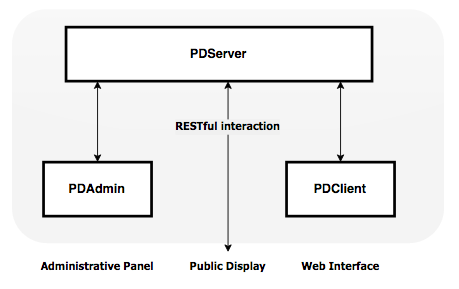
\includegraphics[width=.7\columnwidth]{img/4_implementation/4-overview}
    \end{center}
 \caption{Overview of the PDSurvey platform}
 \label{fig:4-pdsurvey-platform}
\end{figure}

 For administrative purposes we created a RESTful backend (PDBackend), 


which enables the creation, management and distribution of surveys to public displays. Attached to this backend there is the   a responsive client 

backend for administrators (built with Angular.js and Bootstrap) and a simplified version of 


\subsection{Requirements}
\label{4a_requirements}

%%% REQUIREMENTS of PROPOSAL %%%
Analyzing the problem statement and scope of the thesis, the following requirements can be derived:

\begin{enumerate}[itemsep=0pt] 
\item development of a survey tool that allows interactive public display installations to be comprehensively assessed 
\item a web-based survey platform will be implemented that can easily be used to evaluate and compare public displays through different channels 
\item different channels to support: 1) evaluation directly at
the display or 2) through a (mobile) website that allows participation also via a smartphone
or tablet.
\item configuration options for public display owners
\end{enumerate}


%%% TECHNICAL REQUIREMENTS %%%
Requirements derived from the problem statement and scope of the thesis:

\begin{enumerate}
\item JavaScript embed code, for public displays
\item supporting multiple devices: public displays, mobile (smartphone, tablet), desktop
\item responsive web design
\end{enumerate}

Additional requirements, self proposed:
\begin{enumerate}
\item scalable
\item modular / extensible
\item multilingual / internationalization (i18n)
\end{enumerate}



\clearpage

%%% Anforderungen an die Plattform %%%
\subsection{Architecture}
\label{4b_architecture}

\begin{figure}%[btph]
    \begin{center}
        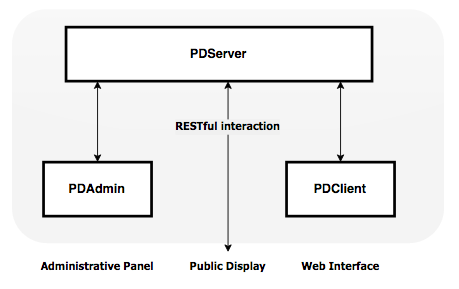
\includegraphics[width=.7\columnwidth]{img/4_implementation/4-overview}
    \end{center}
 \caption{Overview of the PDSurvey platform}
 \label{fig:4-pdsurvey-platform}
\end{figure}


The architecture for the public survey platform can be split into the following five sections:

% Overview, general requirements. Discuss all parts: 
\begin{enumerate}[itemsep=0pt] 
\item Back-end (Node.js, give reasons)
\item Front-end (Responsive)
\item API (REST)
\item Hosting
\end{enumerate}

% + state after each subsubsection why I chose which technologies and why
In the following we will first give an overview of the possible technologies and discuss why I opted for which technology.




%%  PROGRAMMING LANGUAGE  %%
\subsubsection{Programming language}

\paragraph{Categories}

\begin{enumerate}
\item Backend
\item Frontend
\item Mobile
\item Database
\end{enumerate}

% ------------------------------------- % 


\paragraph{Options}


\begin{enumerate}
\item \textbf{JavaScript}

    \begin{itemize}
        \item can be used for all platforms: front-end, back-end, public display
        \item \url{http://www.sitepoint.com/javascript-internet-things/}
        \item \textbf{Front-end}: Reasons why I chose Angular.js and not Backbone.js or Amber.js \url{https://www.airpair.com/js/javascript-framework-comparison}
        \item \textbf{Backend}: Why I chose Node.js
        \item Frameworks in Node.js: Connect, Express, Koa, ... which ones I chose why
        \item Discussion of pro/con Node.js: http://www.heise.de/developer/artikel/2x-Nein-4x-Ja-Szenarien-fuer-Node-js-2111050.html
        \item Prinzip und Verwendung von Middlewares in Node.js (wegen der Internationalisierung und Authentisierung) http://www.heise.de/developer/artikel/REST-Webservices-mit-Node-js-Teil-1-Connect-als-Fundament-1802258.html?view=print

    \end{itemize}
    
\item \textbf{Other languages}

    \begin{enumerate}
    \item PHP
    \item Python
    \item Ruby
    \item Java
    \item ASP.NET
    \end{enumerate}

\end{enumerate}
    





%%  API  %%
\subsubsection{API}

\begin{itemize}
\item REST vs SOAP
\item why I chose REST
\end{itemize}

My REST API Design, using sub-resources \url{http://code.tutsplus.com/tutorials/restful-api-design-with-nodejs-restify--cms-22637}




%%  DATABASE  %%
\subsubsection{Database}

Another fundamental aspect presented the underlying database technology, storing all of the data. A big variety of professional and open-source database management systems (DBMS) already exist on the market, but ...

Criteria for choosing the right DBMS for this project: popularity, size of community, suitability for prototyping, integration with Node.js/Angular.js

% Comparison in between ...

% My choice

Not only due to it's popularity, but also 
% - wanted to learn something new
% - popular in industry
% - MEAN stack


\paragraph{SQL: MySQL}

\begin{enumerate}
\item http://www.mysql.com/
\item "MySQL ist aus gutem Grund das Arbeitstier der Open-Source-Welt geworden: Es bietet viele der M\"oglichkeiten grosser kommerzieller Datenbanken - und ist dabei kostenlos. In seiner aktuelen Form ist MySQL performant und besitzt viele Features." \cite{hughes2012einfuhrung} (Quelle: Buch - Einf\"uhrung in Node.js, Tom Hughes-Croucher \& Mike Wilson, O'Reilly, Seite 134)
\end{enumerate}


\paragraph{SQL: PostgreSQL}

\begin{enumerate}
\item http://www.postgresql.org/
\item "Postgres (sp\"ater PostgreSQL) ist ein objektorientiertes RDBMS, das urspr\"unglich an der University of California in Berkeley entwickelt wurde. Vater des Projekts war Professor Michael Sonebraker, der es als Nachfolger seines \"alteren Ingres-Datenbank-Systems ansah. [...] Nach der Zeit in Berkeley übernahmen Open-Source-Entwickler das Projekt, ersetzten den ursprünglichen QUEL-Sprachinterpreter durch einen SQL-Sprachinterpreter und benannen das Projekt in PostgreSQL um." \cite{hughes2012einfuhrung} (Quelle: Buch - Einf\"uhrung in Node.js, Tom Hughes-Croucher \& Mike Wilson, O'Reilly, Seite 141)
\end{enumerate}


\paragraph{NoSQL: CouchDB}

\begin{enumerate}
\item http://couchdb.apache.org/
\item "CouchDB bietet einen MVCC-basierten (Multi-Version Concurrency Control) Dokumentenspeicher in einer JavaScript Umgebung. Werden Dokumente (Datens\"atze) in CouchDB hinzugef\"ugt oder aktualisiert, dann wird der gesamte Datensatz gespeichert und \"altere Versionen der Daten als obsolet markiert. Diese \"alteren Versionen des Datensazes k\"onnen immer noch in die neueste Version \"ubernommen werden, aber es wird immer eine neue Version erzeugt und f\"ur einen schnellen Lesezugriff in fortlaufenden Speicherbereichen abgelegt" \cite{hughes2012einfuhrung} (Quelle: Buch - Einf\"uhrung in Node.js, Tom Hughes-Croucher \& Mike Wilson, O'Reilly, Seite 113)
\end{enumerate}

\paragraph{NoSQL: Redis}

\begin{enumerate}
\item http://redis.io/
\item "Redis ist eine In-Memory-Datenbank mit einer Schl\"ussel/Wert-Ablage, die Ihnen sehr vertraut vorkommen sollte, wenn Sie schon \"uber Erfahrungen mit Schl\"usse/Wert-Caches wie Memcache verf\"ugen. Redis wird verwendet, wenn Performance und Skalierbarkeit wichtig sind. In vielen F\"allen entscheiden sich die Entwickler daf\"ur, es als Cache f\"ur die von einer relationealen Datenbank wie MySQL empfangenen Daten einzusetzen, auch wenn es deutlich mehr kann." \cite{hughes2012einfuhrung} (Quelle: Buch - Einf\"uhrung in Node.js, Tom Hughes-Croucher \& Mike Wilson, O'Reilly, Seite 121)
\end{enumerate}

\paragraph{NoSQL: MongoDB}

"NoSQL databases came back into the mainstream when developers needed better performance and were ok with giving up the relational aspect of RDBs (unions, joins, etc)" \url{http://psitsmike.com/2012/02/node-js-and-mongo-using-mongoose-tutorial/}

\begin{enumerate}
\item http://www.mongodb.org/
\item MongoDB is document database, storing all data in the form of JavaScript objects, PHP arrays, Python dicts or Ruby hashes. This significantly facilitates the handover from JavaScript to the database management system (DBMS).
\item "Da Mongo eine JavaScript-Umgebung mit BSON-Objektspeichern (einer Bin\"ar-Adaption von JSON) mitbringt, ist das Lesen und Schreiben von Daten aus Node heraus ausgesprochen effizient. Mongo speichert eintreffende Datens\"atze im Speicher, daher ist es in Situationen mit viel Schreibvorg\"angen eine ideale Wahl. Jede neue Version bietet verbessertes Clustering, bessere Replikation und Sharding. Da die eintreffenden Datens\"atze im Speicher abgelegt werden, ist das Einf\"ugen von Daten in Mongo nicht blockierend, womit es ideal f\"ur das Protokollieren von Operationen und Telemetriedaten ist. Mongo unterst\"utzt JavaScript-Funktionen in Abfragen. Dadurch ist es beim Lesen sehr leistungsf\"ahig, so zum Beispiel bei MapReduce-Anfragen. Mit dem dokumentenbasierten Datenspeicher von MongoDB k\"onnen Sie in Eltern-Datens\"atzen auch Kind-Datens\"atze ablegen. So kann zum Beispiel ein Blogartikel mit all seinen Kommentaren in einem einzelnen Datensatz gespeichert werden, wodurch er sich auch wieder sehr schnell auslesen l\"asst."  \cite{hughes2012einfuhrung}
\end{enumerate}

Reasons for using MongoDB
\begin{enumerate}
\item ideal for lots of write procedures
\item non-blocking write operations, ideal for Node.js and for logging data (good for our future work)
\item good read performance
\item good scalability
\item fully supports JSON syntax
\item good integration with Node.js, see Mongoose\footnote{http://mongoosejs.com/}
\end{enumerate}


Notes from the MondoDB University M101JS Class
\begin{enumerate}
\item is non-relational, ideal for JSON data
\item MongoDB is schemaless. Two documents in the same collection can have different schemas.
\item MongoDB provides a good compromise between scalability/performance and the depth of funcitonality
\item Drawback: MongoDB does not support Joins or Transactions
\end{enumerate}



%%  HOSTING  %%
\subsubsection{Hosting}

For the hosting of the platform a free and easy scalable solution was of importance. Our first choice was Heroku\footnote{https://www.heroku.com/}, due to its simplicity of setup, its native support of Node.js and the seamless integration with MongoDB\footnote{https://mongolab.com/}.

% TODO: IaaS vs PaaS: https://www.youtube.com/watch?v=Q8jZHc0NS6A
% give reasons why I chose PaaS (Platform as a Service)

    % Heroku        PaaS
    % IBM BlueMix   PaaS
    % Amawon AWS    IaaS
    % self hosting  IaaS

    %   comparison  http://smashingboxes.com/ideas/heroku-vs-amazon-web-services


Alternative were Google App Engine, IBM BlueMix, Amazon Web Services (Amazon EC2) or hosting everything on local or virtualized machines at our university. However for our scenario all of the above options had their drawbacks in comparison to Heroku. Google App Engine (as of December 2014) still had no native support for Node.js and custom runtimes had to be used to get Node.js support up and running. IBM BlueMix just got overhauled, offered full out-of-the-box Node.js support, however they only the first 30 days were free and the pricing model wasn't as attractive. Amazon Web Services offering a Infrastructure as a Service (IaaS), would have required too much administration of the server, which would have slowed down the main objective of the project, the development of the survey platform. The same goes for the last option, hosting a MEAN-stack environment on our own servers at LMU Munich. All of the above are well-known solutions in the industry, however due to simplicity and ease of use we chose Heroku.



\paragraph{Database}

http://mongoosejs.com/ + https://mongolab.com


\clearpage
\subsection{Modeling}
\label{4c_modeling}

	The model for the \textit{PDSurvey} platform is maintained with the help of the Node package Mongoose. Node.js maps the route parameters and routes all requests to the corresponding Mongoose model. Angular.js builds its model upon the REST API and maps it via dynamic two-way-binding to it's scope. Thus all changes to the model originate from Mongoose.



\subsubsection{Development Process / Modeling}

	The development process of the PDSurvey platform was inspired and influenced by the following approaches:

	\begin{itemize}
	\item working agile and user centered... TODO: look up how to best explain it.

	\item User Centered Design: (paper nr 31): ``constitutes an iterative process of system design, deployment and evaluation'' (quote from paper 31). Work iteratively, continuous deployment and evaluation.

	\item Concept of extreme programming\footnote{\url{http://www.extremeprogramming.org/rules.html} (accessed on November 14, 2014)}: First user stories were written and assessed in a small group. The next step was to transfer these stories to user models, describing in detail which functionality the stakeholders of PDSurvey are supposed to have. Later a first software architecture and software model was built, getting more specific. Dependencies between models were defined and this model was continuously refined and improved throughout the dvelopment phase. The last step of the modeling represented screen designs, getting a clear view of what the interface might later look like.

	\item Used the extreme programming\footnote{\url{http://www.extremeprogramming.org/rules.html} (accessed on November 13, 2014)} approach: user stories, release planning, release schedule, small releases, iterating


	\item criteria for good user stories: http://tigertechtalk.wordpress.com/2012/10/17/wie-schreibe-ich-eine-gute-user-story-und-was-ist-das-uberhaupt/
	\end{itemize}








\subsubsection{User roles}

As of now only two roles are implemented, the admin-role and the guest-role.

% FEEDBACK VON FLORIAN: nein, nicht zu komplex machen. Es sollte sogar reichen, nur zwischen Admin & Operator (= Application Provider) zu unterscheiden, da der end user (das Public Display) ja sowieso nur auf die öffentlichen REST API Zugriff hat. (2014-11-14)


In the long term it would be desirable to have the following user roles: Admin, Operator, Evaluator, DisplayApplication.






\subsubsection{Software model}

In total there are the following classes.

\begin{enumerate}
\item list all classes
\item 1 UML diagram is enough, according to Florian
\end{enumerate}


\subsubsection{Dependencies}

Of special interest are the following four models: Survey, Display, Campaign and Responses.

\paragraph{Surveys:} Surveys resembles the foundation of PDSurvey, with the aim of reuse and standardization. A survey consists of multiple sections, being built of of multiple questions. Each question is of a corresponding question type and every survey belongs to a category. This allows the filtering for relevant surveys. To be able to create private surveys, not being shared across the entire platform, every survey is assigned to an individual user.

\paragraph{Displays:} In the display collection all displays connected to the PDSurvey platform are contained. To allow for an evaluation across multiple display models and based on the context of the displays, the display model and a static and/or dynamic context is assigned to every display.

\paragraph{Campaigns:} Campaigns resemble the most integral part, since they glue all of the pieces together and allow the distribution of surveys to public display networks. A campaign consists of displays and surveys and creates the mapping of the questionnaires to public displays. Additionally to each of those mapping an individual context can be assigned, enabling the later comparison of results in between the public displays.

\paragraph{Responses:} All responses made to each survey are logged in the Response collection. The queries are carried out individually per user, per display and per campaign. This model will be the base for further extensions, amongst others the automatic evaluation of the survey responses and the comparison inbetween an entire display network, to be able to find out which properties of a display might be related to certain effects.

\paragraph{Context:} One of the benefits of creating such a survey platform is being able to collect and evaluate large amounts of data, without having to pay more people for conducting and evaluating the survey. The idea would be to collect a large number of responses from a variety of displays in various settings, and assigning a specific context to every display connected to PDSurvey. Once enough data is collected, having the ability to evaluate and compare the displays between each other. Interesting questions for analysis would be, which role the context plays on how the users behave, when running identical software settings on the displays, but only varying the context (position, size of display, surrounding environment of the display, positioning it outdoors or indoors, influence of the weather, type of building it is positioned in).


\begin{figure}%[btph]
    \begin{center}
        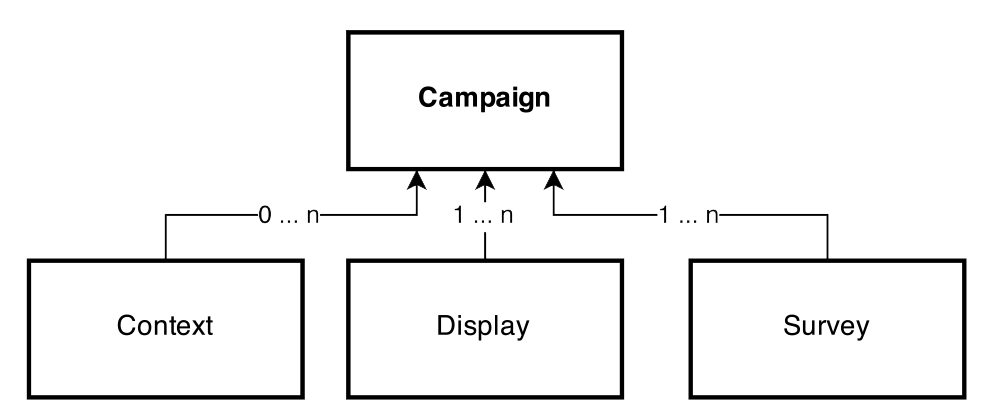
\includegraphics[width=.8\columnwidth]{img/4_implementation/4-dependency-campaign}
    \end{center}
 % \begin{center}\LARGE [BILD]\end{center}
 \caption{Campaign model dependencies}
 \label{fig:4-dependency-campaign}
\end{figure}


++ neue Namensgebung, um in der domain specific language zu bleiben --> application provider / display provider / space provider (anstatt Operator). Wir werden aber nur mit dem Application Provider (anstatt Operator) im System arbeiten





\subsubsection{REST interface}

Defining the REST API. 

% TODO: Explain why I chose which level of separation / detail.

Notes from before I started writing: 
\begin{enumerate}
\item Think about using a Extreme Programming approach http://www.extremeprogramming.org/rules.html
\end{enumerate}

\clearpage
\subsection{Implementation}
\label{4d_implementation}


Briefly describe how I approached the implementation.

\begin{enumerate}
\item Challenges
\item Problems
\item ...
\end{enumerate}


\subsubsection{Package Manager}

\begin{enumerate}
\item NPM and Bower (instead of Browserify) + state reasons
\item State reasons, why I did / didn't check in the code for npm / bower components: \url{http://addyosmani.com/blog/checking-in-front-end-dependencies/}

    \begin{itemize}
    \item "prevent bad dependencies from breaking their app"
    \item "the longevity of package managers and their tooling"
    \item to be independent of other services and thus to garantee a longer life for the tool
    \end{itemize}
\end{enumerate}



\subsubsection{Frontend Framework}

give an overview of current Frontend Frameworks and briefly state which one I used why. A good comparision can be found here \url{http://www.sitepoint.com/5-most-popular-frontend-frameworks-compared/}

\begin{enumerate}
\item Bootstrap
\item Foundation by Zurb
\item ...
\end{enumerate}



\subsubsection{Deployment}

Practical deployment, best practices, how I proceded, and why

\begin{enumerate}
\item GitHub Repo
\item Deployment to Heroku
\end{enumerate}

%\________________________________________________________

\cleardoublepage

    \section{Evaluation}

	\begin{enumerate}
	\item For a good SAMPLE of how to list the basic population (x male, y female) of the survey, have a look at paper number 25 from the Appendix. (WIP)
	\item MOTIVATE: explain why we make this field study, explain what we hope to expect. what are our assumptions. what did we expect from the questionnaires, what did we expect from the interviews?
	\end{enumerate}

	In order to see whether our thoughts regarding the survey platform hold true in practice, we chose to conduct an expert interview with two display providers and also a short field study at our university, deploying surveys to a public display and to tablets.


\subsection{Expert Interview}



\subsection{Field Study}

	The field study took place during the first two weeks of March 2015 in a faculty building of Ludwig-Maximilians-University of Munich. Data was collected on 14 consecutive days and personal semi-structured interviews were carried out on five working days during in the same two weeks. A total of 149 interactions were recorded with the game installed on the public display and 63 survey responses were recorded.

	The goal of this study was to validate the previous thoughts and to see how users use and respond to the survey platform.

\subsubsection{Research Questions}

	The research questions were:

	\begin{itemize}
	\item What motivated our users to fill out surveys?
	\item Which channels are most suited for completing surveys (on a digital platform) in public?
	\item In which situations is the user most willing to answer surveys on public displays?
	\item (not really copious: how many questions are acceptably)
	\item (not really copious: how the users noticed / perceived the survey)
	\end{itemize}

	In addition to these questions we were interested in user stories, which feedback they gave us in regards to answering surveys on screens in the public.

\subsubsection{Study Setup}

	\paragraph{Participants}

	\paragraph{Apparatus}

		Our object of investigation was a large touchscreen with four feedback channels for completing a survey.

		The survey was run on a XXXXX display . The main application installed on the public display was a game called \textit{Balloon Shooter} developed and run by Jiamin Shi, a PhD student at the Group for Media Informatics at LMU Munich.

		\begin{enumerate}
		\item list as detailed information regarding the game as possible
		\item ask Jiamin, whether I can post screenshots of the game?
		\end{enumerate}

	\paragraph{Location}

	Faculty building for computer science, ethnology, political science, japanologie and physics. m,m

	The study setup was in the entrance hall of the university building, .

	% Show Diagram of User paths inside the entrance hall.


\subsubsection{Condition}


\subsubsection{Methodology}

\subsubsection{Results}

	\begin{enumerate}
	\item describe the results from the evaluation
	\item e.g. 1) prefered feedback channel, 2) number of acceptable answers, 3) preferred setting
	\item say which implications this gives for the PDSurvey research platform
	\end{enumerate}

	\paragraph{Quantitative Data}
		asdf


	\paragraph{Qualitative Data}
		asdf


	\begin{enumerate}
	\item TODO: think about what my evaluation has to do with my platform. make sure that this link is clear! Make this link clear in the following summary.
	\end{enumerate}


\subsection{Summary}

	\begin{enumerate}
	\item (summarize the expert interviews)
	\item summarize the quantitative results
	\item summarize the qualitative results 
	\end{enumerate}

%________________________________________________________


\cleardoublepage

    \section{Results}


\begin{enumerate}
\item First present all of the plain observations and findings first, without any personal opinion.
\item MAYBE COMBINE THIS CHAPTER WITH 5. EVALUATION
\end{enumerate}


\subsection{Quantitative Results}

\begin{enumerate}
\item Quantitative: pure facts
\item Qualitative: a combination of facts + evaluation
\end{enumerate}


\subsection{Qualitative Results}

\subsection{Discussion}

Start with a few sentences that summarize the most important results (+ see \url{http://www.ldeo.columbia.edu/~martins/sen_sem/thesis_org.html}).

Now allowing room for interpretation and personal opinions

\subsection{Limitations}

\begin{enumerate}
\item the tablet was always on, it was possible to approach the tablet directly without having the option to participate in the survey via smartphone or email. 
\item the novelty effect played a role for the first part of the evaluation. It was striking to see a response rate of 50 percent. If we exclude all participants who directly accessed the tablet and skipped the appeal to use one of the four options, there was still a response rate of 10 percent.
\end{enumerate}

%________________________________________________________


\cleardoublepage

    \section{Conclusion}

Outlook and future work



\subsection{Summary}

\begin{enumerate}
\item auch Link zu Videodaten loggen können. Die Rohdaten zB in einem Dropbox-Ordner ablegen und mittels einer API oder Dateiname in Ordnerstruktur mit loggen
\end{enumerate}


\subsection{Future Work}


\paragraph{Survey Platform}

	\begin{enumerate}
	\item Logging, adding more data sources
	\end{enumerate}


\paragraph{Evaluation}

	\begin{enumerate}
	\item Number of questions tollerated on each evaluation channel (public display, tablet, smartphone, laptop/desktop)
	\end{enumerate}



%________________________________________________________


\cleardoublepage

\part*{Appendix}
\appendix
\addcontentsline{toc}{part}{Appendix}

% Keine Kopfzeile mehr oben auf jeder Seite
\fancyhead[LE,RO,LO,RE]{}

\section{Content of enclosed CD}

%________________________________________________________

\cleardoublepage

\section{Documentation}

\subsection{User Documentation}

"Most likely others will use your program. Writing a good user's manual will facilitate the use of your program. The important thing is to write for the naive user. It is best to assume that users of your program will know nothing about computers or their interfaces. A clear, concise, step-by-step description of how one uses your program can be of great value not only to others, but to you as well. You can identify awkward or misleading commands, and by correcting these, develop a much more usable product. Start from your requirements document to remind yourself what your program does."

\subsection{Developer Documentation}

\subsubsection{Authentication}

\begin{enumerate}
\item Login mechanisms: good explanation of the differences for Single-Page Applications (SPA) = \url{https://vickev.com/#!/article/authentication-in-single-page-applications-node-js-passportjs-angularjs}
\item + for more information, see Weeks 14 + 16 + 17
\end{enumerate}


During the prototyping phase we also 

For authentication there are the following common approaches, suited for RESTful web services.

\begin{itemize}
\item Token-based authentication: JSON Web Token (JWT)
\item Cookie-based authentication
\item 
\end{itemize}



\subsection{Maintenance Documentation}

"If your work has lasting benefit, someone will want to extend the functionality of your code. A well thought-out maintenance manual can assist in explaining your code. The maintenance manual grows from your specification, preliminary design, and detailed design documents. The manual shows how your program is decomposed into modules, specifies the interfaces between modules, and lists the major data structures and control structures. It should also specify the effective scope of changes to your code."


%________________________________________________________

\cleardoublepage
\part*{Bibliography}
\addcontentsline{toc}{part}{Bibliography}


%%  Literature / BibTex  %%

%%%\begin{thebibliography}{99}

%% Import for 'literature.bib' file
\bibliography{literature}{}

%%%\bibliographystyle{plain}

%%%%% TODOO: remove double heading! %%%%%
%% http://tex.stackexchange.com/a/22654 %%

%%%\bibitem{Ivory01}

%%%  M.\ Y.\ Ivory, M.\ Hearts:
%%%  \href{http://www.ischool.washington.edu/myivory/thesis/thesis.pdf}{%
%%%    An Empirical Foundation for Automated Web Interface Evaluation}.
%%%  Ph.D. thesis, University of California at Berkeley, 2001




%%  Web References  %%
\clearpage

\hspace{-\leftmargin}{\Large\bfseries Web References}

\begin{thebibliography}{99}
\bibliographystyle{plain}

\bibitem{NielsenAlertbox}

  J.\ Nielsen: Alertbox: Current Issues in Web Usability
  \url{http://useit.com/alertbox/}, accessed April~24, 2005.


\end{thebibliography}
\end{document}